\chapter{Crafting}
The Elder Scrolls franchise has featured a number of different crafting systems that allowed you to create weapons, armor, potions, poisons, spells, and enchantments. This chapter is dedicated to describing the crafting systems of the Elder Scrolls Tabletop RPG: Alchemy, Blacksmithing and Enchanting. These all require some calculation, so be sure to have those calculators handy! Fortunately, you will not be doing them often. (Spellmaking is covered in Chapter 6. See section 6.4.1. for details.)\\

\section{Alchemy}
\begin{tcolorbox}
\textbf{Note}: Alchemy is indisputably the most calculation-intensive crafting skill thanks to Bethesda's convoluted system! I have simplified it somewhat, but it still requires you to pay careful attention every time you craft a potion! You've been warned!
\end{tcolorbox}

Alchemy is the art of making potions and poisons. Many substances have latent magical properties that only come out when properly distilled. To create alchemical concoctions, you need a mortar and pestle and at least two ingredients to mix together. You can mix up to four ingredients at once. If two of the ingredients share a property, the resulting mixture will have that property as well. Using more than two ingredients with the same effect will not increase the magnitude or duration of that effect, however; these are determined by skill level and the alchemy equipment you use.\\

This method can be used to discover the properties possessed by the reagents you use. You can also eat a small portion of a single ingredient to learn that ingredient's most prominent properties. This is called \textit{wortcraft}. As your Alchemy skill improves, your wortcraft will allow you to detect more properties from individual reagents. You may also learn some alchemical properties from recipes or books. Seek out your local alchemist for more information. It is recommended you keep an alchemy notebook detailing the known properties of reagents.

\subsection{Potion or Poison?}
In the Elder Scrolls series, some factor determines whether your alchemical concoction qualifies as a potion or a poison, which affects whether you drink it or apply it to your weapon when used. The factor varies by game. In the Elder Scrolls Tabletop, there is no hard difference between potions and poisons. In fact, any concoction can be drunk or applied to a weapon if you wish. You could drink a Damage Health poison or apply a Restore Health potion to an arrow if you really wanted to.

\subsection{Alchemy Apparatuses}
While the mortar and pestle is the only alchemy apparatus you need to craft a potion, there are other types of apparatuses you can use to improve upon its effects. Each type comes in five quality levels, the use of which is restricted by current Alchemy level: Novice, Apprentice, Journeyman, Expert and Master. Each quality level has a value used in the alchemy equations. The following values apply to each apparatus:

\begin{center}
{
\rowcolors{2}{gray!25}{white}
\begin{tabular}{ll}
	Novice & 0.1\\
	Apprentice & 0.25\\
	Journeyman & 0.5\\
	Expert & 0.75\\
	Master & 1\\
\end{tabular}
}
\end{center}

\subsubsection{Mortar and Pestle}

\begin{wrapfigure}{R}{0.1\textwidth}
	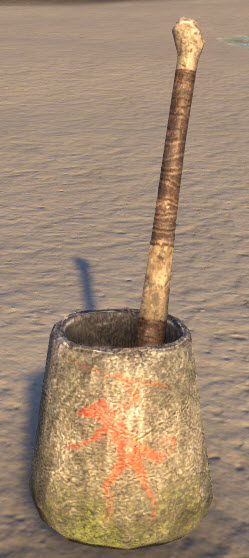
\includegraphics[width=\textwidth]{mortarpestle.png}
\end{wrapfigure}

This apparatus consists of a hard bowl made of stone, ceramic or hard wood (the mortar) and a heavy, blunt, club-shaped object (the pestle). Reagents are placed into the mortar and then ground into a fine mixture which is then stirred into water to create a potion. The mortar and pestle are required to craft any potion or poison.\\

The magnitude and duration of each effect of mixtures produced using only a mortar and pestle are called the \textit{base magnitude} and \textit{base duration}. These are used as intermediate values when other apparatuses are involved; otherwise, they are the true magnitude and duration of the mixture. Base magnitude and duration are calculated with the following formulas:

\begin{itemize}
	\item $\text{Base Magnitude}=(\frac{\text{Alchemy Skill}+25*\text{MortarPestleQuality}}{0.4*\text{EffectBaseCost}})^{1/2.28}$
	\item $\text{Base Duration}=4*\text{Base Magnitude}$
\end{itemize}

Certain potion effects do not come with a magnitude, such as water breathing. Dispel effects likewise do not come with a duration. For these special cases, use the following formulas instead:

\begin{itemize}
	\item $\text{Base Magnitude}=(\frac{\text{Alchemy Skill}+\text{MortarPestleQuality}*25}{0.1*\text{EffectBaseCost}})^{1/1.28}$
	\item $\text{Base Duration}=\frac{\text{Alchemy Skill}+\text{MortarPestleQuality}*25}{0.1*\text{EffectBaseCost}}$
\end{itemize}

\begin{tcolorbox}
\textbf{Note}: I am not sure whether the exponent difference is a typo or not. If your potion magnitude seems off, try using the other exponent and see if it makes more sense. Let me know if this comes up in game.
\end{tcolorbox}

The value \textit{MortarPestleQuality} is taken from the list in the previous subsection. The value used for \textit{Effect Base Cost} comes from which types of effects the potion will have. Ask your GM for the value needed or consult the following link: \url{http://en.uesp.net/wiki/Oblivion:Spell_Effects}

\subsubsection{Retort}
\begin{wrapfigure}{L}{0.2\textwidth}
	\includegraphics[width=\textwidth]{retort.png}
\end{wrapfigure}

A retort is a roughly spherical vessel with a long, downward-pointing neck. It is typically made of glass, though it may also be made of metal. Retorts are used to distill liquids by allowing vapors to condense in the neck, after which they flow downward into a collection vessel placed underneath.\\

If you use a retort in your concoction, it will increase the magnitude and duration of all positive effects. Magnitudes are increased by $50\%*\text{Quality}$. Durations are increased by $100\%*\text{Quality}$.

\subsubsection{Calcinator}

\begin{wrapfigure}{R}{0.2\textwidth}
	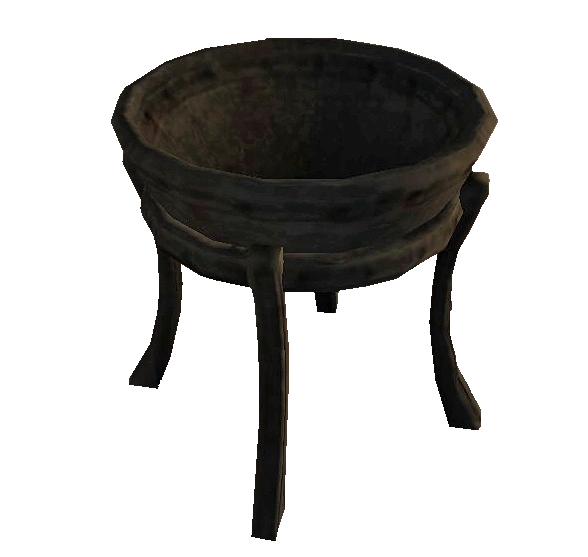
\includegraphics[width=\textwidth]{calcinator.png}
\end{wrapfigure}

A calcinator is a metal bowl on a ring stand. An alchemical mixture is placed into it above an open flame, heating it to temperatures at which some compounds in the mixture decompose or transition into other forms.\\

Using a calcinator in your concoction will increase the magnitude and duration of both positive and negative effects. The magnitude and duration of positive effects are increased by $35\%*\text{Quality}$, and the magnitude and duration of negative effects are increased by $140\%*\text{Quality}$.

\subsubsection{Alembic}

\begin{wrapfigure}{L}{0.2\textwidth}
	\includegraphics[width=\textwidth]{alembic.png}
\end{wrapfigure}

An alembic consists of two glass vessels joined by a downward-sloping tube. The mixture is heated in one vessel, producing vapors which collect at the top of the tube and flow into the collection vessel. The only difference between this and a retort is that the retort has the tube joined with the top of the heated vessel, suggesting the game developers did not think thoroughly about their choice of alchemy apparatuses. In fact, retorts are often part of an alembic.\\

Regardless, using an alembic will increase the magnitude and duration of your mixture's negative effects. Magnitudes are increased by $50\%*\text{Quality}$. Durations are increased by $100\%*\text{Quality}$.

\subsubsection{Using Multiple Apparatuses}
When you use multiple apparatuses in a potion, the modifying percentages are added before being applied to the base magnitude and duration. For example, a positive effect will increase by 240\% when a master retort and calcinator are used.

\subsubsection{Selling Potions}
Potions are often a great way of making money. The base cost for each potion you make is equal to $0.45(\text{Alchemy Skill}*25*\text{MortarPestleQuality})$.

\section{Blacksmithing}

The \textit{Elder Scrolls V: Skyrim} was the first entry in the franchise to introduce a crafting system for weapons and armor. In previous titles, the Armorer skill was only used to repair items. Since the Elder Scrolls Tabletop is primarily based on the mechanics of Morrowind and Oblivion, the blacksmithing system is made from scratch to provide a simple, sensible way to create weapons and armor.

\begin{figure}[H]
	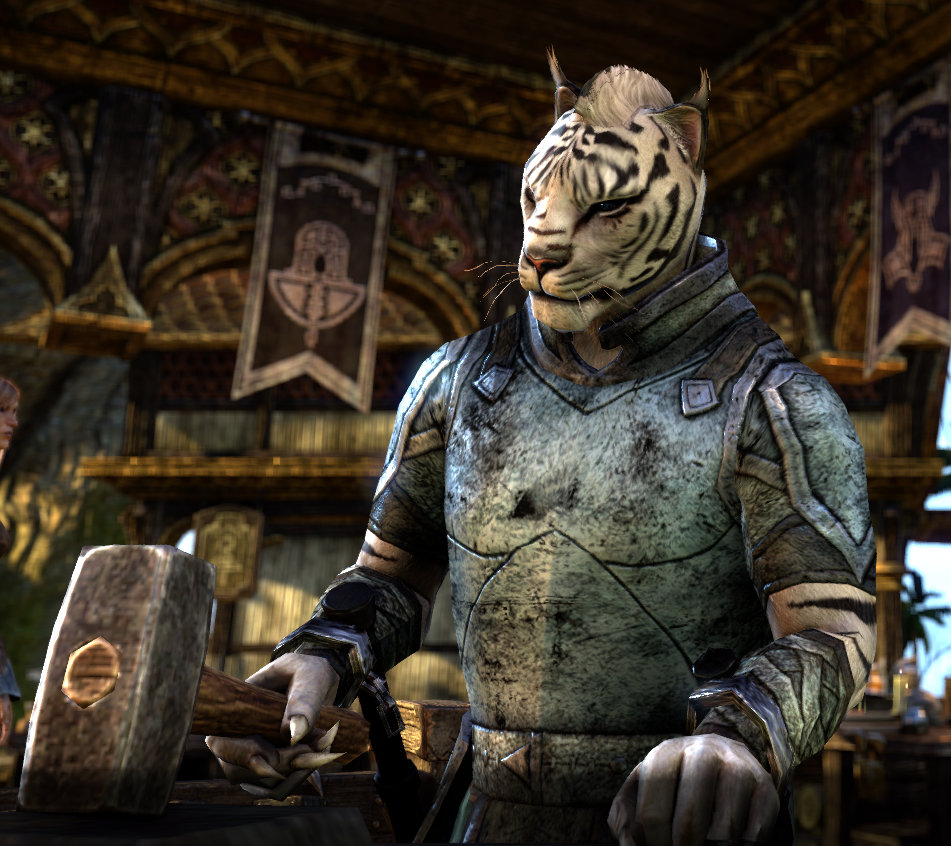
\includegraphics[width=0.65\textwidth]{blacksmith.png}
\end{figure}

\subsection{Requirements}
Unlike in Skyrim, the Elder Scrolls Tabletop does not require that you collect a set of components necessary to craft an item. Rather, the GM will specify a gold cost for crafting the item which is assumed to cover the expenses of acquiring the components. Blacksmithing can be very expensive!\\

Certain narrative conditions may be required before you can craft an item. Does your character have the knowledge needed to smith with a certain material or in a certain style? Are you able to find or purchase all the materials you need, or are some items completely unavailable? Sometimes, narrative conditions can reduce the cost of crafting an item as well. For example, if you collected a lot of Dwemer metal while exploring a Dwemer ruin, crafting Dwemer metal items should not cost as much. Work with your GM to decide the conditions affecting your ability to create items.\\

When you have met all conditions, you need access to a forge and enough time to work. Don't expect to craft items in a dungeon.

\section{Enchanting}

Enchanting is the art of applying persistent magical effects to items. Enchanted items are highly sought after by most cultures in Tamriel for a multitude of reasons. For example, their effects are constant and do not drain magicka when used, they can be used by people without magical training and they are immune to dispel effects. Weapons with enchantments have a limited number of charges, though they may be recharged by spell merchants or by using filled soul gems. Enchanted weapons also gain the Magic property, even when their enchantment charges are depleted. Beware, however: blacksmiths cannot repair enchanted items unless their Armorer skill is Journeyman level or higher.

\subsection{Requirements}
To begin enchanting, you must first gain access to an enchanting altar. These are significantly more common than spellmaking altars and may be found in places such as Mages Guild buildings or wizards' homes. Once you have access to an enchanting altar, you need a soul gem with a trapped soul and an item to receive the enchantment. You may place any magical effect on the item if it is the effect of a spell you know and can cast. You also get to name the item. Certain spell effects cannot be used as enchantments. For example, worn items cannot be enchanted with healing effects. Spell effects may be denied for enchantment at the GM's discretion.\\

With all these things, you may perform a one-hour ritual to carry out the enchantment. Various other components are needed, the cost of which is equal to the base effect cost (ask your GM or see \url{http://en.uesp.net/wiki/Oblivion:Spell_Effects}) times the magnitude of the effect. Only one effect can be placed on an item at a time. If you perform the enchantment ritual on an item that is already enchanted, its enchantment is overwritten by the new one. The base value of an enchanted item increases by the magnitude of the effect multiplied by the effect's barter factor (see \url{http://en.uesp.net/wiki/Oblivion:Spell_Effects}).

\subsection{Soul Gems}

Soul gems are special magic crystals that can be used to capture the souls of living creatures when they die. Once filled, they can be used to apply enchantments or recharge enchanted items. Soul gems come in six quality levels:
Petty, Lesser, Common, Greater, Grand, and Black.\\

Creature souls come in five sizes that correspond with soul gem types: Petty, Lesser, Common, Greater and Grand. A soul gem can hold souls of equal or lesser size. The souls of intelligent creatures (humanoids and the like) always count as Grand, but they may only be stored in black soul gems. This practice is illegal and is considered a form of necromancy. Nevertheless, it is possible.

\begin{wrapfigure}{L}{0.3\textwidth}
	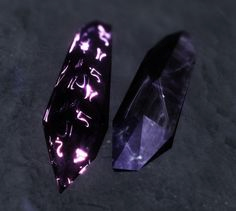
\includegraphics[width=\textwidth]{soulgem.png}
\end{wrapfigure}

Capturing a soul is quite simple: if the target dies while affected by a Soul Trap effect and you have a soul gem capable of holding its soul, you may choose to fill the soul gem with it. Soul Trap effects can be applied by spells or even enchanted weapons.\\

When a soul gem is used for enchanting or recharging, the crystal breaks and cannot be reused. A soul gem with a soul inside cannot contain another soul, nor can the trapped soul be discarded and replaced.

\subsection{Weapon Enchantments}
Weapon enchantments have a certain amount of magicka stored in them and expend a certain amount of magicka each time they are used. The amount of magicka spent is determined by the spell cost formula described in section 6.4.1; it depends on magnitude and effect. You get to choose the magnitude of the enchantment you place on a weapon so long as the resulting cost does not exceed 85. The maximum amount of magicka stored in a weapon enchantment is determined by the level of the soul used to enchant the item. The magicka value of each soul level is as follows:

\begin{center}
{
\rowcolors{2}{gray!25}{white}
\begin{tabular}{ll}
	Petty & 150 magicka\\
	Lesser & 300 magicka\\
	Common & 800 magicka\\
	Greater & 1200 magicka\\
	Grand & 1600 magicka\\
\end{tabular}
}
\end{center}

Therefore, the number of uses is determined by the charge of the item divided by the magicka cost of the effect. A maximum magnitude enchantment made with a grand soul would therefore have 18 charges, for example.\\

Whenever you use a soul to recharge an item, it regains magicka equal to the size of the soul used. For example, a weapon with a charge of 1000/1600 that is recharged with a petty soul will end up with 1150/1600 magicka.\\

\subsection{Worn Enchantments}
Enchantments can also be placed on clothing, jewelry and armor. Worn enchantments do not expend charge but rather have a constant effect that is always active so long as you are wearing the item. The effect magnitude of worn item enchantments cannot be chosen, but is rather a product of the soul level used to create it. To determine the magnitude of the enchantment, ask your GM or consult the table at \url{http://en.uesp.net/wiki/Oblivion:Enchanting#Worn_Enchantments}.

\begin{figure}
	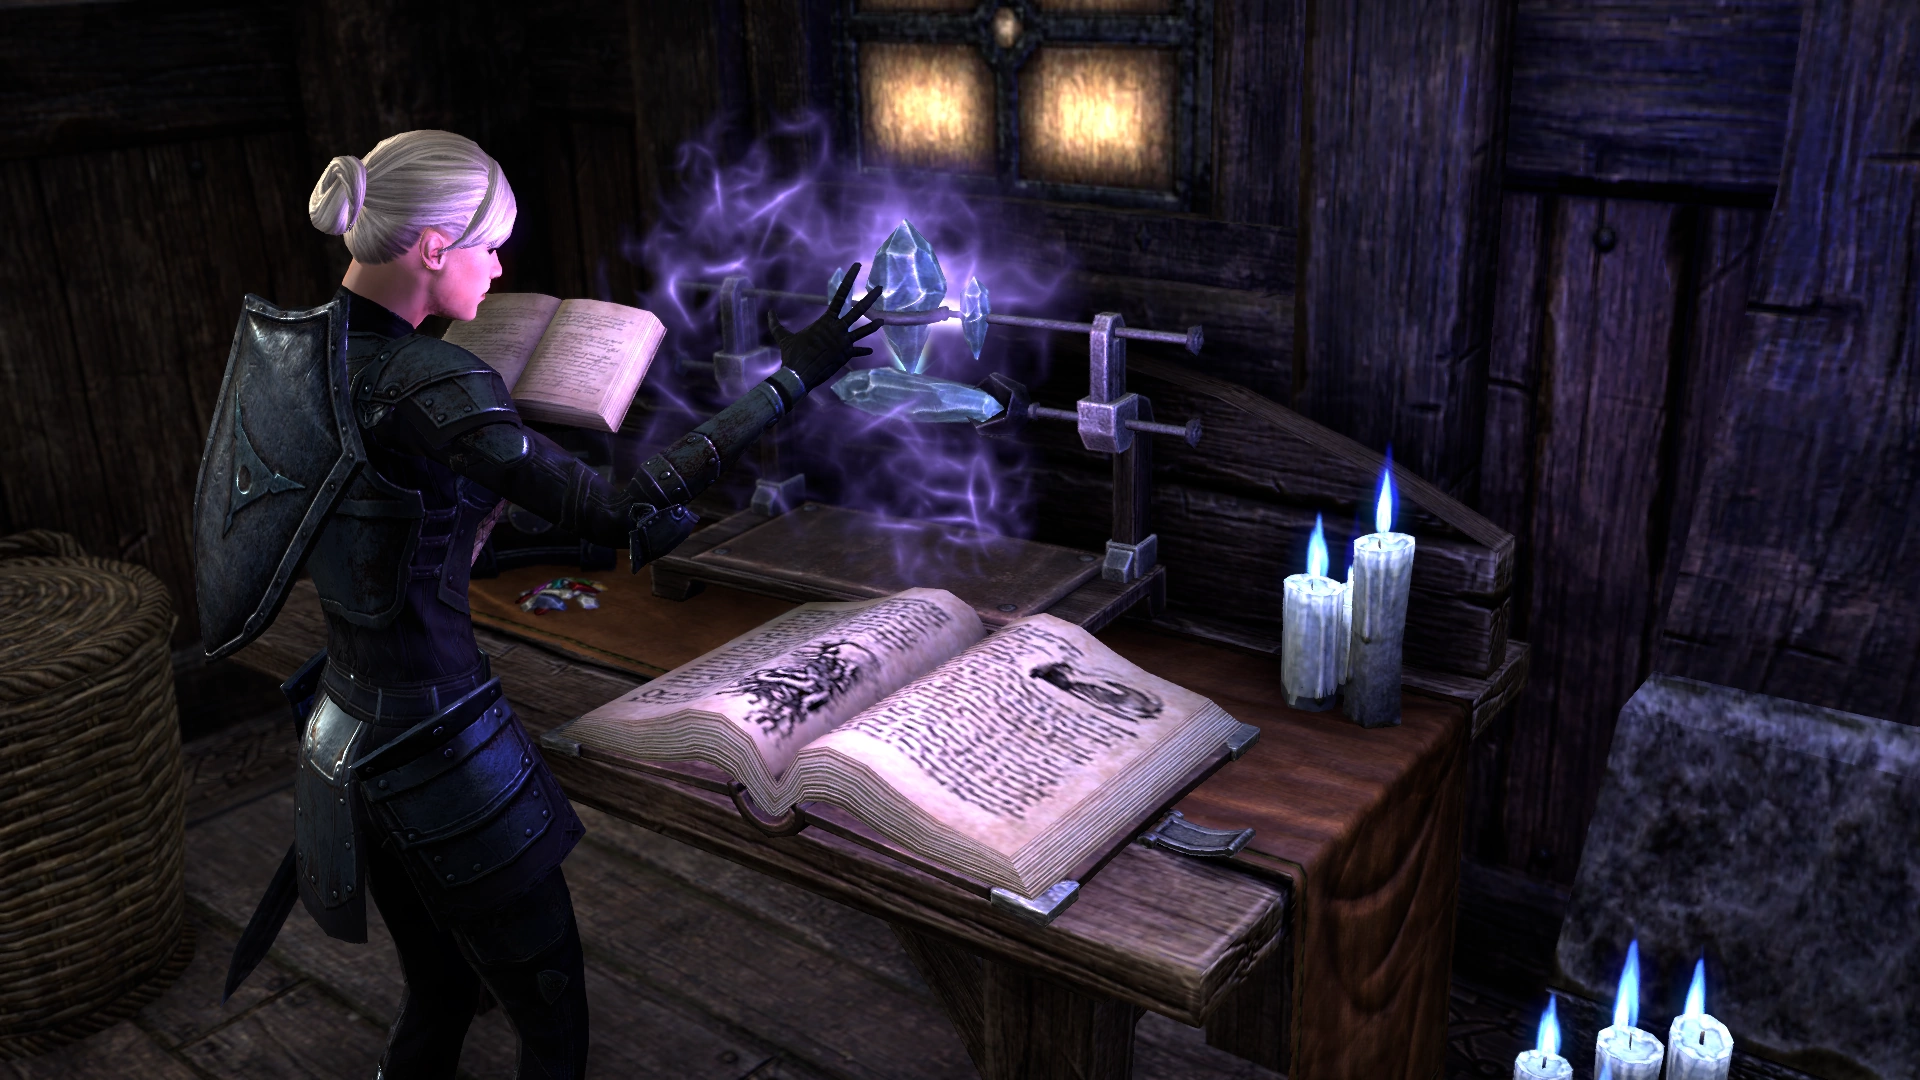
\includegraphics[width=\textwidth]{Enchanting.png}
\end{figure}
